\section{Методы сжатия без потерь}

Данные восстанавливаются с точностью до бита, что не приводит к каким-либо потерям информации. Однако, сжатие без потерь показывает обычно худшие степени сжатия.


\subsection{Алгоритм Хаффмана}

Алгоритм Хаффмана — жадный алгоритм оптимального префиксного кодирования алфавита с минимальной избыточностью. Был разработан в 1952 году аспирантом Массачусетского технологического института Дэвидом Хаффманом при написании им курсовой работы. Используется во многих программах сжатия данных, например, PKZIP 2, LZH и др.

Построение кода Хаффмана сводится к построению соответствующего бинарного дерева по следующему алгоритму:

\begin{figure}[H]
    \centering
    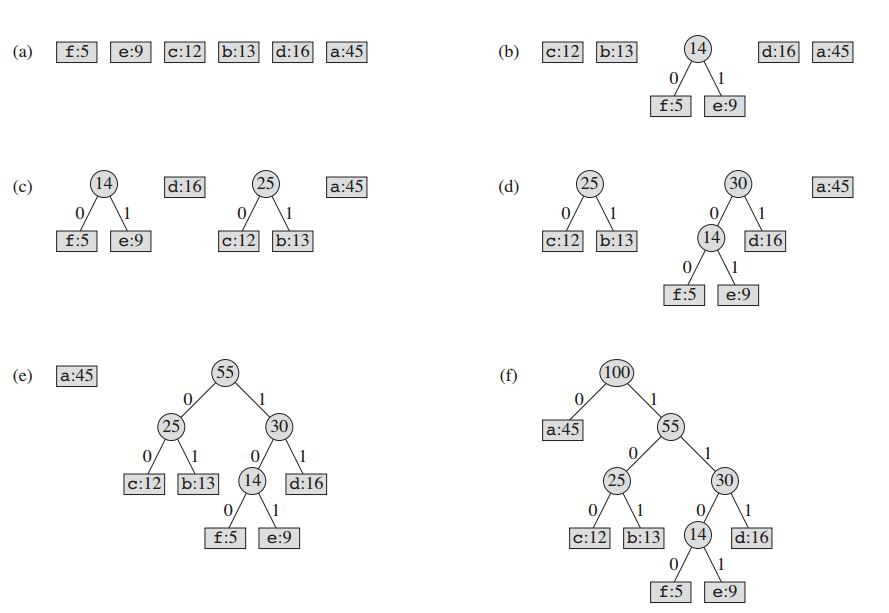
\includegraphics[width=.9\textwidth]{img/haffman.jpg}    
    \caption{пример работы алгоритма Хаффмана для алфавита ABCDEF}
\end{figure}


\begin{enumerate}
\item Составим список кодируемых символов, при этом будем рассматривать один символ как дерево, состоящее из одного элемента c весом, равным частоте появления символа в строке.
\item Из списка выберем два узла с наименьшим весом.
\item Сформируем новый узел с весом, равным сумме весов выбранных узлов, и присоединим к нему два выбранных узла в качестве детей.
\item Добавим к списку только что сформированный узел вместо двух объединенных узлов.
\item Если в списке больше одного узла, то повторим пункты со второго по пятый.
\end{enumerate}


\begin{figure}[!h]
    \lstinputlisting[language=Python,caption=пример реализации на Python]{source/haffman.py}
\end{figure}
  


\subsection{Арифметическое кодирование}

Алгоритм сжатия информации без потерь, который при кодировании ставит в соответствие тексту вещественное число из отрезка $[0;1)$. Данный метод, как и алгоритм Хаффмана, является энтропийным, то есть длина кода конкретного символа зависит от частоты встречаемости этого символа в тексте. Арифметическое кодирование показывает более высокие результаты сжатия, чем алгоритм Хаффмана, для данных с неравномерными распределениями вероятностей кодируемых символов.

В отличие от алгоритма Хаффмана, не имеет жесткого постоянного соответствия входных символов группам бит выходного потока. Это даёт алгоритму большую гибкость в представлении дробных частот встречаемости символов.

Как правило, превосходит алгоритм Хаффмана по эффективности сжатия, позволяет сжимать данные с энтропией, меньшей 1 бита на кодируемый символ, но некоторые версии имеют патентные ограничения от компании IBM.


\begin{figure}[H]
    \centering
    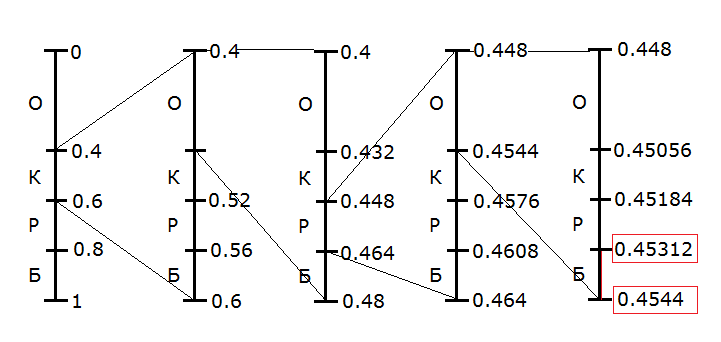
\includegraphics[width=.9\textwidth]{img/arif.png}    
    \caption{пример работы алгоритма арифметического кодирования для алфавита БКОР}
\end{figure}


\textbf{Кодирование}: на вход алгоритму передаются текст для кодирования и список частот встречаемости символов.

\begin{enumerate}
\item Рассмотрим отрезок $[0;1)$ на координатной прямой.
\item Поставим каждому символу текста в соответствие отрезок, длина которого равна частоте его появления.
\item Считаем символ из входного потока и рассмотрим отрезок, соответствующий этому символу. Разделим этот отрезок на части, пропорциональные частотам встречаемости символов.
\item Повторим пункт (3) до конца входного потока.
\item Выберем любое число из получившегося отрезка, которое и будет результатом арифметического кодирования.
\end{enumerate}

\textbf{Декодирование}: алгоритм по вещественному числу восстанавливает исходный текст.

\begin{enumerate}
\item Выберем на отрезке [0;1), разделенном на части, длины которых равны вероятностям появления символов в тексте, подотрезок, содержащий входное вещественное число. Символ, соответствующий этому подотрезку, дописываем в ответ.
\item Нормируем подотрезок и вещественное число.
\item Повторим пункты 1—2 до тех пор, пока не получим ответ.
\end{enumerate}

\begin{figure}[!h]
    \lstinputlisting[language=Python,caption=пример реализации на Python]{source/arif.py}
\end{figure}
  



% \subsection{LZ77}

% LZ77 и LZ78 — алгоритмы сжатия без потерь, опубликованные в статьях Абрахама Лемпеля и Якоба Зива в 1977 и 1978 годах. Эти алгоритмы наиболее известны в семействе LZ*, которое включает в себя также LZW, LZSS, LZMA и другие алгоритмы. Оба алгоритма относятся к алгоритмам со словарным подходом. 

% LZ77 использует так называемое <<скользящее окно>>. Основная идея заключается в том, чтобы кодировать одинаковые последовательности элементов. Т.е., если во входных данных какая-то цепочка элементов встречается более одного раза, то все последующие её вхождения можно заменить «ссылками» на её первый экземпляр.

% \begin{figure}[H]
%     \caption{Пример <<скользящего окна>>}
%     \centering
%     
\includegraphics[width=.9\textwidth]{img/lz77-1.png}    
% \end{figure}

% Алгоритм LZ77 выдает коды, состоящие из трех элементов:

% \begin{enumerate}
% \item смещение в словаре относительно его начала подстроки, совпадающей с содержимым буфера;
% \item длина подстроки;
% \item первый символ в буфере, следующий за подстрокой.
% \end{enumerate}


% \subsection{LZMA}

% LZMA (англ. Lempel-Ziv-Markov chain-Algorithm) — алгоритм сжатия данных, разрабатываемый с 2001 года. Используется в архиваторе 7-Zip для создания сжатых архивов в формате 7z.

% Алгоритм основан на схеме сжатия данных по словарю, сходной с использованной в LZ77, и обеспечивает высокий коэффициент сжатия (обычно превышающий коэффициент, получаемый при сжатии с использованием bzip2), а также позволяет использовать словари различного размера (до 4 Гб).

% \begin{figure}[H]
%     \caption{Принцип работы алгоритма LZMA}
%     \centering
%     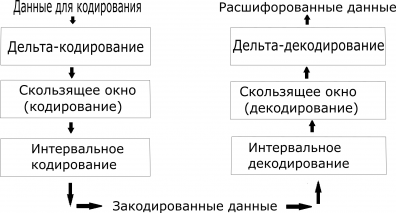
\includegraphics[width=.9\textwidth]{img/lzma-1.png}    
% \end{figure}

% Дельта фильтр перестраивает входные данные для эффективного сжатия скользящим окном. Первый байт на выходе совпадает с первым байтом на входе, последующие же байты представлены как разность между текущим и предыдущим байтом. Для постоянно меняющихся данных, дельта-кодирование делает работу скользящего окна более эффективной.

% \textbf{Кодирование}:

% Функция принимает массив и длину массива как аргументы, если длина не была передана, то массив не обрабатывается.
% Инициализируем переменные tmp, для сохранения последнего элемента и last для хранения предыдущего числа.Инициализируем цикл.
% В цикле:
% 3.1 Сохраняем элемент с индексом i.
% 3.2 Вычисляем разницу между элементом под номером i и i−1 и перезаписываем ее в элемент массива с индексом i.


% \subsection{Deflate}

% Deflate — это алгоритм сжатия без потерь, использующий комбинацию алгоритмов LZ77 и Хаффмана. Изначально был описан Филом Кацем для второй версии его архиватора PKZIP, который впоследствии был определён в RFC 1951 (1996 год).

% Deflate считается свободным от всех существующих патентов, и пока оставался в силе патент на LZW (он применяется в формате GIF), это привело к использованию Deflate не только в формате ZIP, для которого Кац изначально его спроектировал, но также в компрессоре/декомпрессоре gzip и в PNG-изображениях.

% Закодированные в соответствии с форматом Deflate данные представля­ют собой набор блоков, порядок которых совпадает с последовательностью соответствующих блоков исходных данных. Используется 3 типа блоков за­кодированных данных:

% \begin{enumerate}
%     \item состоящие из несжатых данных;
%     \item использующие фиксированные коды Хаффмана;
%     \item использующие динамические коды Хаффмана.
% \end{enumerate}

% Длина блоков первого типа не может превышать 64 Кб, относительно других ограничений по размеру нет. Каждый блок типа 2 и 3 состоит из двух частей:
% \begin{itemize}
% \item описания двух таблиц кодов Хаффмана, использованных для кодирова­ния данных блока;

% \item собственно закодированных данных.
% \end{itemize}

% Коды Хаффмана каждого блока не зависят от использованных в преды­дущих блоках.

% Само описание динамически создаваемых кодов Хаффмана является, в свою очередь, также сжатым с помощью фиксированных кодов Хаффма­на, таблица которых задается форматом.

% Алгоритм словарного сжатия может использовать в качестве словаря часть предыдущего блока (блоков), но величина смещения не может быть больше 32 Кб. Данные в компактном представлении состоят из кодов эле­ментов двух типов:
% \begin{itemize}
    
% \item литералов (одиночных символов);

% \item указателей имеющихся в словаре фраз; указатели состоят из пары <длина совпадения, смещение>
% \end{itemize}

% Длина совпавшей строки не может превышать 258 байт, а смещение фразы - 32 Кб. Литералы и длины совпадения кодируются с помощью од­ной таблицы кодов Хаффмана, а для смещений используется другая табли­ца; иначе говоря, литералы и длины совпадения образуют один алфавит. Именно эти таблицы кодов и передаются в начале блока третьего типа.

% \textbf{Алгоритм декодирования}